\chapter{提案システム}
本章では,本研究で開発したスマートフォンのモーションセンサを利用した個人認証システムについて説明する.

\section{システムの概要}
本システムは,Android端末に一般的に搭載されている加速度センサと角速度センサを用いてモーションデータを収集し,Denoising Autoencoderとその後ろに識別用ニューロンを繋げた識別器を用いて個人認証を行う.
本システムには,登録モードと認証モードという二つの動作モードがある.
登録モードでは,入力されたモーションデータの一部をランダムにデータの最大値及び最小値でノイズを付与したものを用いてDenoising Autoencoderで特徴を学習させる.
その後識別用ニューロンを繋いで入力データに対する教師信号として0.0を,入力データと同じ値域・次元数で乱数生成したダミーデータに対する教師信号として1.0を与えて識別器の学習を行う.
認証モードでは,入力されたモーションデータを学習済みの識別器に入力し,得られた出力を用いて個人認証を行う.

\subsection{動作モード選択}
Androidアプリケーションを起動すると,図\ref{start}のスタート画面が表示される.
画面下部にある``Start''ボタンを押すことで,図\ref{select-mode}の動作モード選択ダイアログが表示される.
``Registration''を選択すると登録モードに,``Authentication''を選択すると認証モードに遷移する.

% @suppress DuplicatedSection
\subsection{登録モード}
登録モードに遷移すると,図\ref{reg-input-name}のユーザ名入力画面が表示される.
ここでは登録するユーザ名を入力する.
ユーザ名を入力して画面下部にある``OK''ボタンを押すことでユーザ名が正しく入力されたか確認する処理が行われ,確認できれば図\ref{registration}のモーション入力画面が表示される.
ユーザ名が入力されていない,もしくは空白文字しか入力されていない場合は図\ref{reg-input-name-toast}のようにAndroidシステムに標準で用意されている通知機能であるToastを用いてユーザにエラーを通知する.

モーション入力画面では,画面下部の``モーションデータ取得''ボタンを押している間,加速度センサと角速度センサそれぞれにデータを取得するための専用スレッドが起動して各センサからデータが取得・蓄積される.
また,データ取得用スレッドの起動と同時に時間計測用スレッドも起動し,1秒経過毎に端末をバイブレートさせることでユーザにモーション入力の経過時間を伝える.
モーション入力中に任意のタイミングで``モーションデータ取得''ボタンから指を離すことで,モーション入力を終了できる.
モーション入力はデフォルトでは3回となっているが,画面右上のハンバーガーメニュー,もしくは端末に搭載されたメニューボタンを押すことで表示される図\ref{reg-menu}のメニュー画面から,``データ取得回数設定''を選択することで回数を変更できる.
``データ取得回数設定''を選択すると,図\ref{reg-change-time}のダイアログが表示される.
画面上にあるスライダーを操作して左右に動かすことで,データ取得回数を増減でき,画面下部の``OK''ボタンを押すことで設定が反映される.
また,先ほどのメニュー画面から``リセット''を選択すると,図\ref{reg-reset}のダイアログが表示される.
ここで``YES''を選択することで,モーションデータの取得状態をリセットし,一からモーション入力をやり直すことができる.

モーション入力が終わるたびに,取得したモーションデータのデータ数が確認される.
加速度センサ及び角速度センサから得られたX軸データのいずれかのデータ数が10個を下回っていた場合,図\ref{reg-recollect}のダイアログを表示し,ユーザに再度モーションを入力させる.
設定回数分のモーション入力が終わると図\ref{reg-progress}のプログレスダイアログが表示され,後述するモーションデータの加工及び識別器の学習を行うスレッドが起動する.

モーションデータの加工及び識別器の学習が終わると図\ref{reg-finish}のダイアログが表示される.
``OK''ボタンを押すことでユーザ名と暗号化した学習済み識別器のパラメータ,データの次元数を他アプリからの読み書きができない形で端末に保存し,スタート画面に遷移する.
何らかの原因で識別器の学習ができなかった場合は図\ref{reg-error}のダイアログが表示される.
``OK''ボタンを押すことでモーションデータの取得状態がリセットされるので再度モーションを入力する.

% @suppress DuplicatedSection
\subsection{認証モード}
認証モードに遷移すると,図\ref{auth-input-name}のユーザ名入力画面が表示される.
ここでは認証するユーザ名を入力する.
ユーザ名を入力して画面下部にある``OK''ボタンを押すことで登録モードで保存されたユーザ名のリストから入力されたユーザ名と合致するものが存在するか検索され,存在していた場合は図\ref{authentication}のモーション入力画面が表示される.
存在していなかった場合は,図\ref{auth-input-name-toast}のようにToastを用いてユーザにエラーを通知する.

モーション入力画面では,画面下部の``モーションデータ取得''ボタンを押している間,加速度センサと角速度センサそれぞれにデータを取得するための専用スレッドが起動して各センサからデータが取得・蓄積される.
また,データ取得用スレッドの起動と同時に時間計測用スレッドも起動し,1秒経過毎に端末をバイブレートさせることでユーザにモーション入力の経過時間を伝える.
モーション入力中に任意のタイミングで``モーションデータ取得''ボタンから指を離すことで,モーション入力を終了できる.
モーション入力は1回となっており,登録モードと違い変更はできない.

モーション入力が終わると,取得したモーションデータのデータ数が確認される.
加速度センサ及び角速度センサから得られたX軸データのいずれかのデータ数が10個を下回っていた場合,図\ref{auth-recollect}のダイアログを表示し,ユーザに再度モーションを入力させる.
設定回数分のモーション入力が終わると図\ref{auth-progress}のプログレスダイアログが表示され,後述するモーションデータの加工及び識別器による個人認証を行うスレッドが起動する.

モーションデータの加工及び個人認証が終わると,認証結果をダイアログで表示する.
認証に成功すれば図\ref{auth-succeed}のダイアログが表示され,``OK''ボタンを押すことでスタート画面に遷移する.
認証に失敗すれば図\ref{auth-failure}のダイアログが表示され,``OK''ボタンを押すことでモーションデータの取得状態がリセットされ,再度個人認証を行える.

\section{モーションデータの加工}
登録モードと認証モードのいずれも,モーションセンサから得られたデータはニューラルネットワークで用いる前に,``データ数の均一化''・``フーリエ変換を用いたローパスフィルタ''・``角速度から変位,角速度から角度への変換''・``変位データを角度データで回転''という四つの加工を行う.

\subsection{データ数の均一化}
本システムでは,モーション入力を任意の時間で行える.
この際,登録モードにおけるデフォルトでは3回のモーション入力によるモーションデータ,認証モードでは登録時に用いたモーションデータと新たに入力されたモーションデータ間でデータ数の差異が生じる場合がある.
本システムで用いたニューラルネットワークでは入力されるデータにおける次元数のばらつきは許容できないため,事前にデータ数を均一化する必要がある.

登録モードでは,最も入力時間の長かったデータを基準に他のデータに対して末尾にゼロを補填する方法を用いる.
認証モードでは,登録時に用いたデータの長さを基準に新たに入力されたデータが短い場合は末尾にゼロを補填し,長い場合は末尾を切り落とす方法でデータ数を均一化している.

% @suppress ParagraphNumber InvalidSymbol
\subsection{ローパスフィルタ}
モーションを入力している際に生じる手の震えなどによるモーションデータへの影響を抑えるために,フーリエ変換を用いたローパスフィルタ処理を実装している.
時間軸領域で表されるデータをフーリエ変換を用いて周波数領域に変換すると,モーション入力中に生じた手の震えなどによるデータが高周波成分として現れる.
この高周波成分を取り除いた上で元の時間軸領域で表されるデータに逆変換するローパスフィルタ処理を行うことで,手の震えなどによる影響の少ないデータを得られる.

フーリエ変換の実装には,CERNのColt Project\cite{4-colt-project}で開発された科学技術計算用ライブラリであるColtをマルチスレッド化したParallel Colt\cite{4-parallel-colt}に含まれている,JTransforms\cite{4-jtransforms}を用いた.

この処理をソースコード\ref{source-lowpass}に示す.

\lstinputlisting[caption=ローパスフィルタ, label=source-lowpass, style=MyJava]{Code/lowpass.java}

% ローパスフィルタの比較グラフ
ローパスフィルタ処理によるデータの変化を示したグラフを図\ref{graph-lowpass}に示す.

\begin{figure}[hbtp]
  \centering
  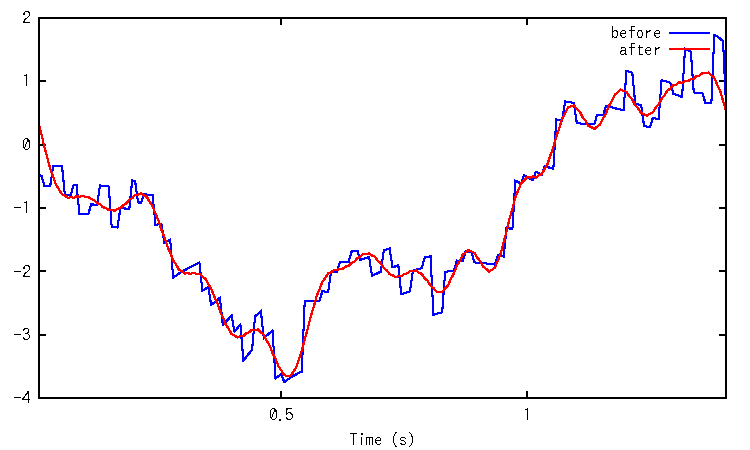
\includegraphics[bb=0 0 360 216, width=12cm]{Graphs/lowpass.pdf}
  \caption{ローパスフィルタ処理によるデータの変化}
  \label{graph-lowpass}
\end{figure}

青色で示した線がローパスフィルタ処理前のグラフ,赤色で示した線が処理後のグラフである.

% @suppress ParagraphNumber InvalidSymbol
\subsection{加速度から変位,角速度から角度への変換}
% ドリフトの影響があるため,足し合わせていく処理はしない
ローパスフィルタ処理したデータに対して,次に加速度から変位,角速度から角度に変換する処理を行う.
加速度から変位への変換は式\ref{accel-to-displacement}で行う.
\begin{equation}
\label{accel-to-displacement}
x = \frac{1}{2} a t^2.
\end{equation}

$x$は変位を,$a$は加速度を,$t$は加速度データの取得間隔を表している.
なお,本システムでは初速度を考慮しない.
この処理をソースコード\ref{source-accel-to-displacement}に示す.

\lstinputlisting[caption=加速度から変位への変換, label=source-accel-to-displacement, style=MyJava]{Code/accelToDisplacement.java}

また,角速度から角度への変換は式\ref{gyro-to-angle}で行う.
\begin{equation}
\label{gyro-to-angle}
y = g t.
\end{equation}

$y$は角度を,$g$は角速度を,$t$は角速度データの取得間隔を表している.
その処理をソースコード\ref{source-gyro-to-angle}に示す.

\lstinputlisting[caption=角速度から角度への変換, label=source-gyro-to-angle, style=MyJava]{Code/gyroToAngle.java}

% @suppress InvalidSymbol
\subsection{変位データを角度データで回転}
加速度から変位,角速度から角度へ変換したデータに対して,次は変位データを角度データで回転させる処理を行う.
この処理をソースコード\ref{source-rotate-vector}に示す.

\lstinputlisting[caption=変位データの角度データを用いた回転,合成, label=source-rotate-vector, style=MyJava]{Code/rotateVector.java}

変位データを回転させるcombineメソッドには,変位データの他にモーションデータ取得開始時点からどれだけ回転したかを保持するangleX・angleY・angleZのラジアンを渡している.
この際,各軸を中心に反時計回りで変位データを回転させるために,それぞれの正負を逆にした上でそのラジアンを求めている.

combineメソッドでは,渡されたラジアンについてそれぞれ$\sin$と$\cos$を求め,式\ref{rotate-matrix}の回転行列を用いてX軸・Y軸・Z軸の順に回転させている.

\begin{eqnarray}
\label{rotate-matrix}
R_x(\theta) = \left(
    \begin{array}{ccc}
        1 & 0 & 0 \\
        0 & \cos\theta & -\sin\theta \\
        0 & \sin\theta & \cos\theta
    \end{array}
\right). \nonumber \\
R_y(\theta) = \left(
    \begin{array}{ccc}
        \cos\theta & 0 & \sin\theta \\
        0 & 1 & 0 \\
        -\sin\theta & 0 & \cos\theta
    \end{array}
\right). \nonumber \\
R_z(\theta) = \left(
    \begin{array}{ccc}
        \cos\theta & -\sin\theta & 0 \\
        \sin\theta & \cos\theta & 0 \\
        0 & 0 & 1
    \end{array}
\right).
\end{eqnarray}

\section{ニューラルネットワークによる学習と識別}
本システムは,図\ref{system-nn}のようなDenoising Autoencoderと識別用ニューロンを繋げたニューラルネットワークにより個人認証を行う.


\begin{figure}[hbtp]
  \centering
  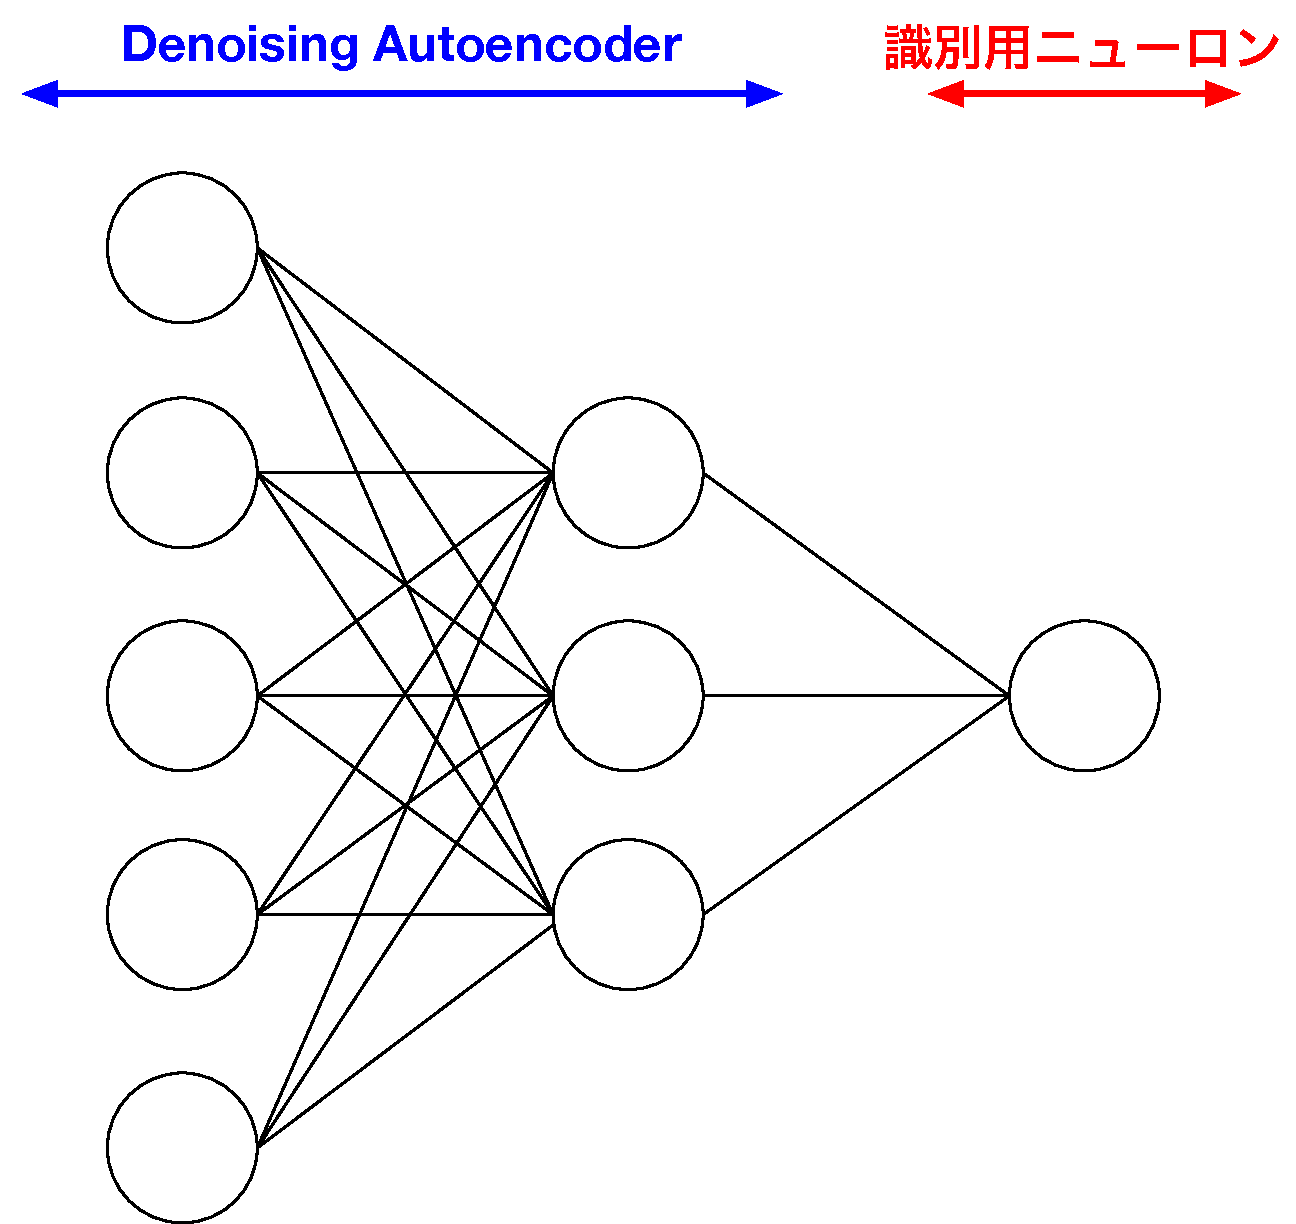
\includegraphics[bb=0 0 622 587, width=9cm]{Figures/system-nn.pdf}
  \caption{識別に用いるニューラルネットワーク}
  \label{system-nn}
\end{figure}

本システムでは,基本的にNVIDIA製GPUを搭載しCUDA\cite{4-cuda}を利用したGPGPUによる高速演算が可能な計算機上で動作するプログラム(以下,サーバ)でニューラルネットワークに関する処理を実行する.
Android端末上で動作するプログラム(以下,クライアント)とサーバでデータをやりとりする際にはTCPソケットを用いる.

% @suppress ParagraphNumber DuplicatedSection InvalidSymbol
\subsection{登録モード}
登録モードでは,動作モード値・ユーザ名・前述の加工を行ったモーションデータをTCPソケットを用いてサーバに送信する.
サーバ側ではこれらデータをJavaで書かれたプログラムで受信し,JNI\cite{4-jni}を用いてC++で書かれたニューラルネットワークプログラムに処理を移す.

ニューラルネットワークプログラムでは,まずDenoising Autoencoderの学習を行う.
%入力データにノイズをのせて学習
まず,受け取ったモーションデータを平均が0,分散が1になるように正規化する.
この処理をソースコード\ref{source-normalize}に示す.

\lstinputlisting[caption=モーションデータの正規化処理, label=source-normalize, style=MyCpp]{Code/normalize.cpp}

そして,正規化した各モーションデータのそれぞれ40\%に,そのデータの最大値あるいは最小値で上書きするノイズ加工を行う.
この処理をソースコード\ref{source-dA-noise}に示す.

\lstinputlisting[caption=dA学習時のノイズ加工, label=source-dA-noise, style=MyCpp]{Code/dA-noise.cpp}

ノイズ加工を行った後,中間層のニューロン数を入力層や出力層のニューロン数から30\%削減し,中間層の活性化関数にシグモイド関数,出力層の活性化関数に恒等関数を用いたDenoising Autoencoderを構築する.
訓練データにノイズ加工を行ったモーションデータを,教師信号にノイズ加工を行う前のモーションデータを与え,損失関数に最小二乗誤差を用いて500回の学習を行う.
また,訓練時に中間層ニューロンのうち50\%をランダムにDropoutさせる.

%学習が完了したら,次は識別用ニューロンをつないで,ダミーデータを生成して学習する
Denoising Autoencoderの学習が終われば,Denoising Autoencoderのパラメータを固定して,この後ろに活性化関数にシグモイド関数を用いたニューロンを繋げる.
そして,正規化する前のモーションデータにおける最大値と最小値の範囲内で生成したランダム値からなるダミーデータを生成し,正規化する.
%こちらもDropout率や学習回数などを
訓練データに正規化したモーションデータとダミーデータを,教師信号にそれぞれ0.0と1.0を与え,損失関数に交差エントロピー誤差を用いて誤差が0.1未満になるまで最大10000回の学習を行う.
この際Dropoutを無効にし,Denoising Autoencoderの出力に対して1から先ほどの学習時に適用したDropout率を引いた0.5を掛ける.

%学習できたら,学習済みニューラルネットワークのパラメータをAndroid端末側に送り返す
学習が終われば,ニューラルネットワークにおける各層ごとのニューロンが持つパラメータを文字列として連結したデータをクライアントに送る.

%Android端末側でうけとって,保存してetc
クライアント側はこのデータを受け取り,暗号化した上で他アプリからの読み書きができない形で保存する.

% @suppress DuplicatedSection
\subsection{認証モード}
認証モードでは,動作モード値・ユーザ名・前述の加工を行ったモーションデータ・登録モードにおいて保存した学習済みニューラルネットワークのパラメータをTCPソケットを用いてサーバに送信する.
サーバ側ではこれらデータをJavaで書かれたプログラムで受信し,JNIを用いてC++で書かれたニューラルネットワークプログラムに処理を移す.

ニューラルネットワークプログラムでは,まず受け取ったモーションデータを平均が0,分散が1になるように正規化する.
次に,受け取った学習済みニューラルネットワークのパラメータをもとにニューラルネットワークを構築する.
構築できたらこれに正規化したモーションデータを与え,出力値を得る.
そして,得られた出力値をクライアントに送る.

クライアント側はこの値を受け取り,値が0.2未満であれば認証成功とし,0.2以上であれば認証失敗とする.

また,認証モードに限り,端末が何らかの理由でサーバに接続できない場合は,ニューラルネットワークの処理に多少時間がかかるが端末のローカルでサーバと同等の処理が行えるようにしている.
